\section{Car Tablet}
We have already shown the mobile app user interface in the RASD, so in this section we will show some mock-ups of the tablet that is present in every car.

\begin{figure}
    \vspace*{-2cm}
    \makebox[\linewidth]{
        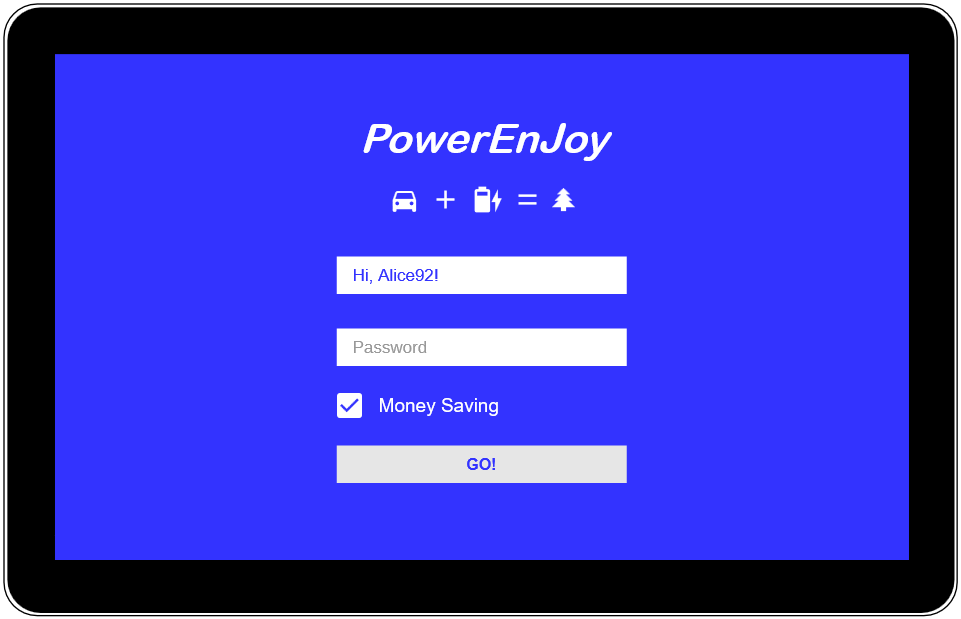
\includegraphics[width=1.3\linewidth]{ui_design/car_login.png}
    }
    \caption{Car login page.}
	\label{fig:car_login}
\end{figure}

When the user enters the car, the screen in figure \ref{fig:car_login} is what he/she will see in the tablet. The tablet receives the nickname of the user that unlocked the car, so it is able to display it. If the password is correct than the user can turn on the car.

\begin{figure}
    \vspace*{-2cm}
    \makebox[\linewidth]{
        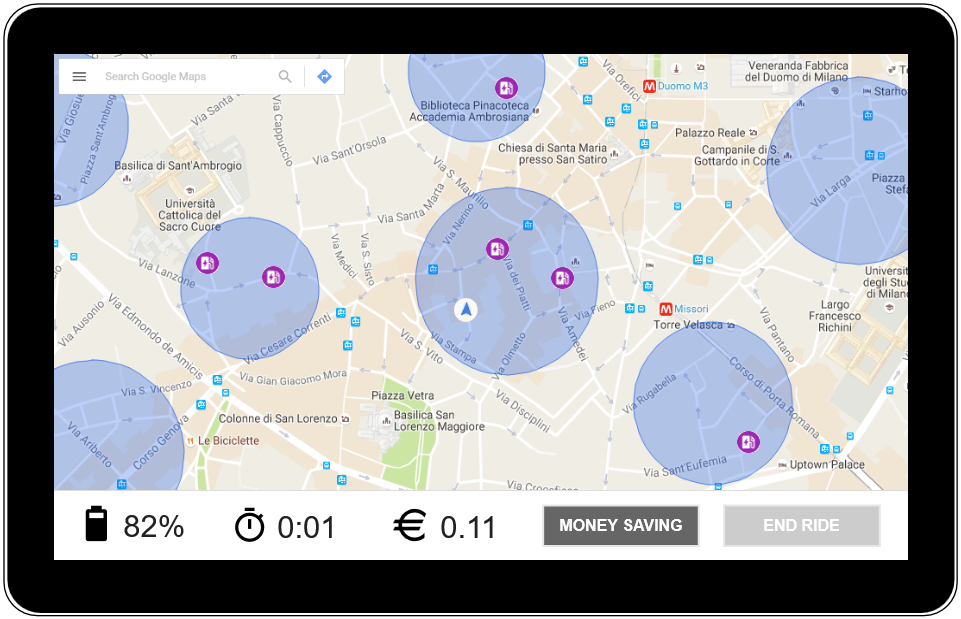
\includegraphics[width=1.3\linewidth]{ui_design/car_main.png}
    }
    \caption{Car main page.}
	\label{fig:car_main}
\end{figure}

If the authentication phase is successful, then on the tablet appears the Main Page. The mock-up of this screen is presented in figure \ref{fig:car_main}. Here you can navigate through the map, where you can find also the safe areas and the power grid stations. In the bar at the bottom, you can find the current percentage of the battery level of the car, the time since the reservation started, the current fee and the buttons to activate the money saving option and to end the ride.

In this picture the money saving option is off and the end ride is disabled because the user is not in a safe area. When the user is in a safe area the button becomes red. Using the search bar, the user can select a destination and set the navigation.

If he/she do so, the screen of the tablet will be something similar to figure \ref{fig:car_ride}. In this example the money saving button is blue, so it means that this option is activated.

\begin{figure}
    \vspace*{-2cm}
    \makebox[\linewidth]{
        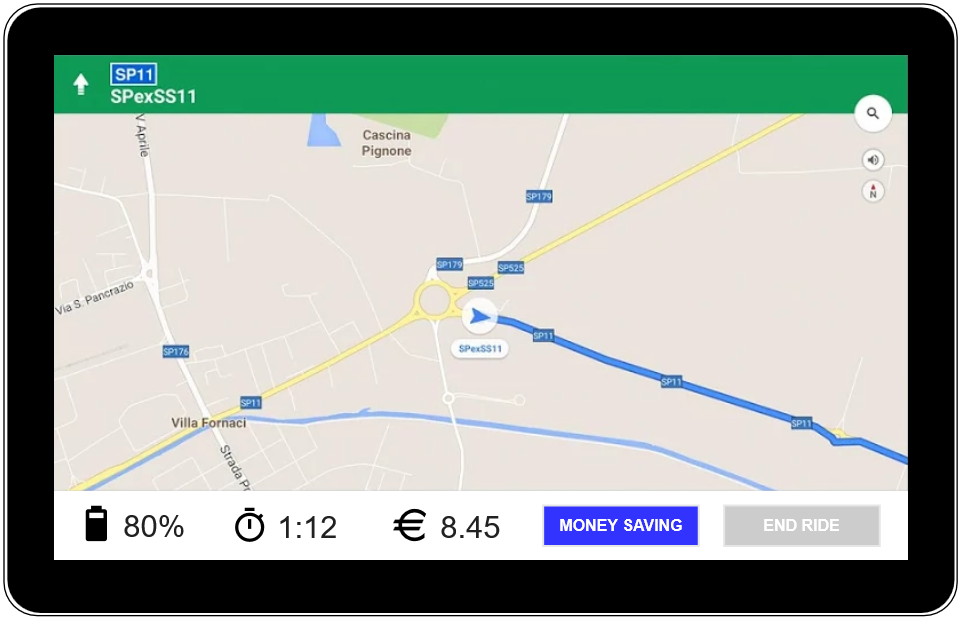
\includegraphics[width=1.3\linewidth]{ui_design/car_ride.png}
    }
    \caption{Car main page.}
	\label{fig:car_ride}
\end{figure}
